\documentclass{article}
% translate with >> pdflatex -shell-escape <file>

% This file is used as unit test for pgfplots, copyright by Christian Feuersaenger.
% 
% See
%   http://pgfplots.sourceforge.net/pgfplots.pdf
% for pgfplots.
%
% Any required input files (for <plot table> or <plot file> or the table package) can be downloaded
% at
% http://www.ctan.org/tex-archive/graphics/pgf/contrib/pgfplots/doc/latex/
% and
% http://www.ctan.org/tex-archive/graphics/pgf/contrib/pgfplots/doc/latex/plotdata/

\usepackage{pgfplots}
\pgfplotsset{compat=newest}

\pagestyle{empty}

\begin{document}
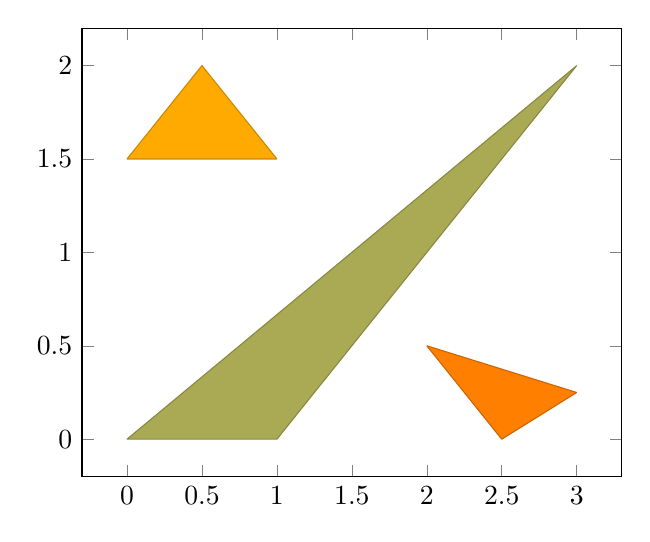
\begin{tikzpicture}
		\begin{axis}
			
		\addplot[patch,point meta=\thisrow{c}] table[row sep=\\] {
			x y c\\
			0 0 0\\
			1 0 0 \\
			3 2 2\\
			%\\
			0 1.5  1.5\\
			1 1.5  1.5\\
			0.5 2  2\\
			%\\
			2.5 0     1\\
			3 	0.25  2\\
			2 0.5     3\\
		}; 
		\end{axis}
	\end{tikzpicture}
\end{document}
